\chapter{Analysis}\label{C:analysis} 
The core of this empirical study is the analysis of corpora of code written in each of the investigated languages. This analysis makes use of many static code analysis methods including:
\begin{itemize}
	\item ANTLR
	\item grep
	\item JSClassFinder
	\item Esprima
\end{itemize}
Each of these tools helps to extract valuable information from one of more of the languages analysed in this study.

\section{Assembling Corpora}
Each language analysed in this study required a corpus of code representative of the ways programmers in the real world are using that language. In the case of Java, prior studies have resulted in the creation of The Qualitas Corpus which is a large collection of open source projects written in the Java language~\cite{QualitasCorpus}. \newline
For the other studied languages, JavaScript, Python, Lua, and Scala, quality existing corpora could not be found. For each of these languages, the top 25 open source projects were sourced from GitHub's "Trending this month" list. This source was chosen because it provides a particularly up to date snapshot of development in each language which ensures that the analysis performed will be as relevant as possible to modern software development.

\section{Java}
The intent in analysing the Qualitas Corpus of Java code is to determine the extent to which developers are making use of Java's inbuilt language features and what developers are doing to work around these language features. Specifically, a Java developers' usage of class inheritance will represent them conforming to the classical inheritance model encouraged by the Java language. In contrast, instances of code which model call forwarding or call delegation will represent cases where the developer could have expressed themselves more concisely through other object inheritance models where delegation and forwarding are supported natively. \newline
Finding occurrences of classical inheritance in Java is as simple as looking for the extends keyword with a grep search. Finding examples of delegation and forwarding is more difficult and requires more information about the syntax tree of the program. To achieve this, each program of the corpus was passed through ANTLR which parses each file according to a Java grammar and constructs an abstract syntax tree which can then be traversed to search for relevant patterns. \newline \newline
The process for extracting statistics from a Java project follows a pipeline structure where each file is parsed and analysed in isolation. The resulting statistics of each file are then aggregated to form the overall statistics across the projects. This file isolation is important because the syntax trees produced by ANTLR consume large amounts of memory so it is not possible to hold all the Java files for a project in memory simultaneously.
\newline
\newline
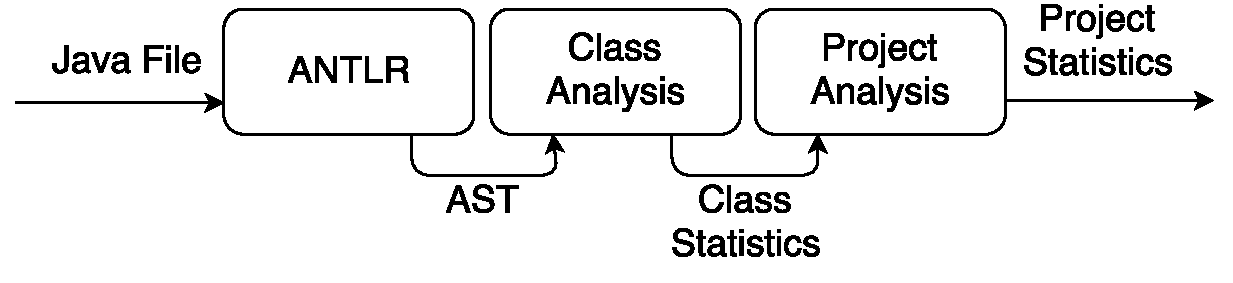
\includegraphics[scale=0.70]{AntlrPipeline.pdf}
\newline
\newline
After each project has been parsed and analysed, the results are then further aggregated to produce corpus level analysis which can be found in the following table:
\newline
\newline
\begin{tabular}{|l|l|l|l|}
	\hline
	& Count  & \% of classes & \% of extended classes \\ \hline
	Total classes                                                                                   & 116427 &               &                        \\ \hline
	Classes extend another class                                                                    & 71203  & 61.16\%       &                        \\ \hline
	Classes are extended by another class                                                           & 20751  & 17.82\%       &                        \\ \hline
	Classes with forwarding                                                                         & 7087   & 6.09\%        &                        \\ \hline
	\begin{tabular}[c]{@{}l@{}}Classes with forwarding\\ that extend another class\end{tabular}     & 3381   & 2.90\%        &                        \\ \hline
	Classes with downcalls in constructors                                                          & 16101  & 13.83\%       &                        \\ \hline
	Classes storing this in constructors                                                            & 2392   & 2.05\%        &                        \\ \hline
	\begin{tabular}[c]{@{}l@{}}Classes with downcalls or\\ storing this in constructor\end{tabular} & 17099  & 14.69\%       &                        \\ \hline
	\begin{tabular}[c]{@{}l@{}}Extended classes with\\ downcalls in constructors\end{tabular}       & 1545   & 1.33\%        & 7.45\%                 \\ \hline
	\begin{tabular}[c]{@{}l@{}}Extended classes storing\\ this in constructors\end{tabular}         & 178    & 0.15\%        & 0.86\%                 \\ \hline
	Classes with delegation                                                                         & 5183   & 4.45\%        &                        \\ \hline
\end{tabular}

\section{JavaScript}
The JavaScript analysis of this study makes extensive use of the prior work in developing the JSClassFinder application~\cite{JSClassFinder}. The aim here is to find the cases where JavaScript developers are deliberately circumventing the native delegation support of the language and are instead modelling their programs with classical inheritance structures.

\section{Timeline}
\begin{ganttchart}[
	hgrid style/.style={draw=black!5, line width=.75pt},
	vgrid={*{6}{draw=none},dotted},
	x unit=0.9mm,
	time slot format=isodate
	]{2016-07-08}{2016-11-11}
	14
	\gantttitlecalendar{month=shortname} \\
	\ganttgroup{Language Analysis}{2016-07-08}{2016-09-01}\\
		\ganttbar{JavaScript}{2016-07-08}{2016-07-21}\\
		\ganttbar{Python}{2016-07-22}{2016-08-04}\\
		\ganttbar{Scala}{2016-08-05}{2016-08-18}\\
		\ganttbar{Lua}{2016-08-19}{2016-09-01} \\
	\ganttgroup{Collective Analysis}{2016-09-02}{2016-10-13}\\
		\ganttbar{Comparing Analyses}{2016-09-02}{2016-09-23}\\
		\ganttbar{Final Report}{2016-09-02}{2016-10-13}\\
	\ganttgroup{Presentation}{2016-10-14}{2016-11-11}\\
		\ganttbar{Creating Presentation}{2016-10-14}{2016-10-27}\\
		\ganttbar{Rehearsing Presentation}{2016-10-28}{2016-11-11}
\end{ganttchart}












